\subsection{OpenStack for IaaS}

OpenStack is an open source Cloud Management solution that utilizes hypervisor-based virtualization technology and provides functions for management of virtualized entities from a central control center. The logical architecture of OpenStack [4] is as below. A typical openstack deployment uses a central controller node with replication and runs all the essential services. Depending on the scale of deployment, these services can either be run on individual nodes or on separate nodes. The services are connected through a common messaging and database architecture and the services are referenced as endpoints. The core computational entities are compute nodes which run agents that communicate with the controller services and host the virtual machines. The controller provides a Graphical User Interface and Command Line Interface to interact with all the services and resources connected to the combined cluster. 

OpenStack is completely written in Python and exposes REST-based APIs which helps integrate with multiple Orchestration or other solutions that need to use OpenStack services and events. OpenStack also integrates with several open source and proprietary underlay technologies for compute, storage and networking through mechanism drivers that are open source components. This is essential for interoperability with existing and new technologies used in enterprise production environments.

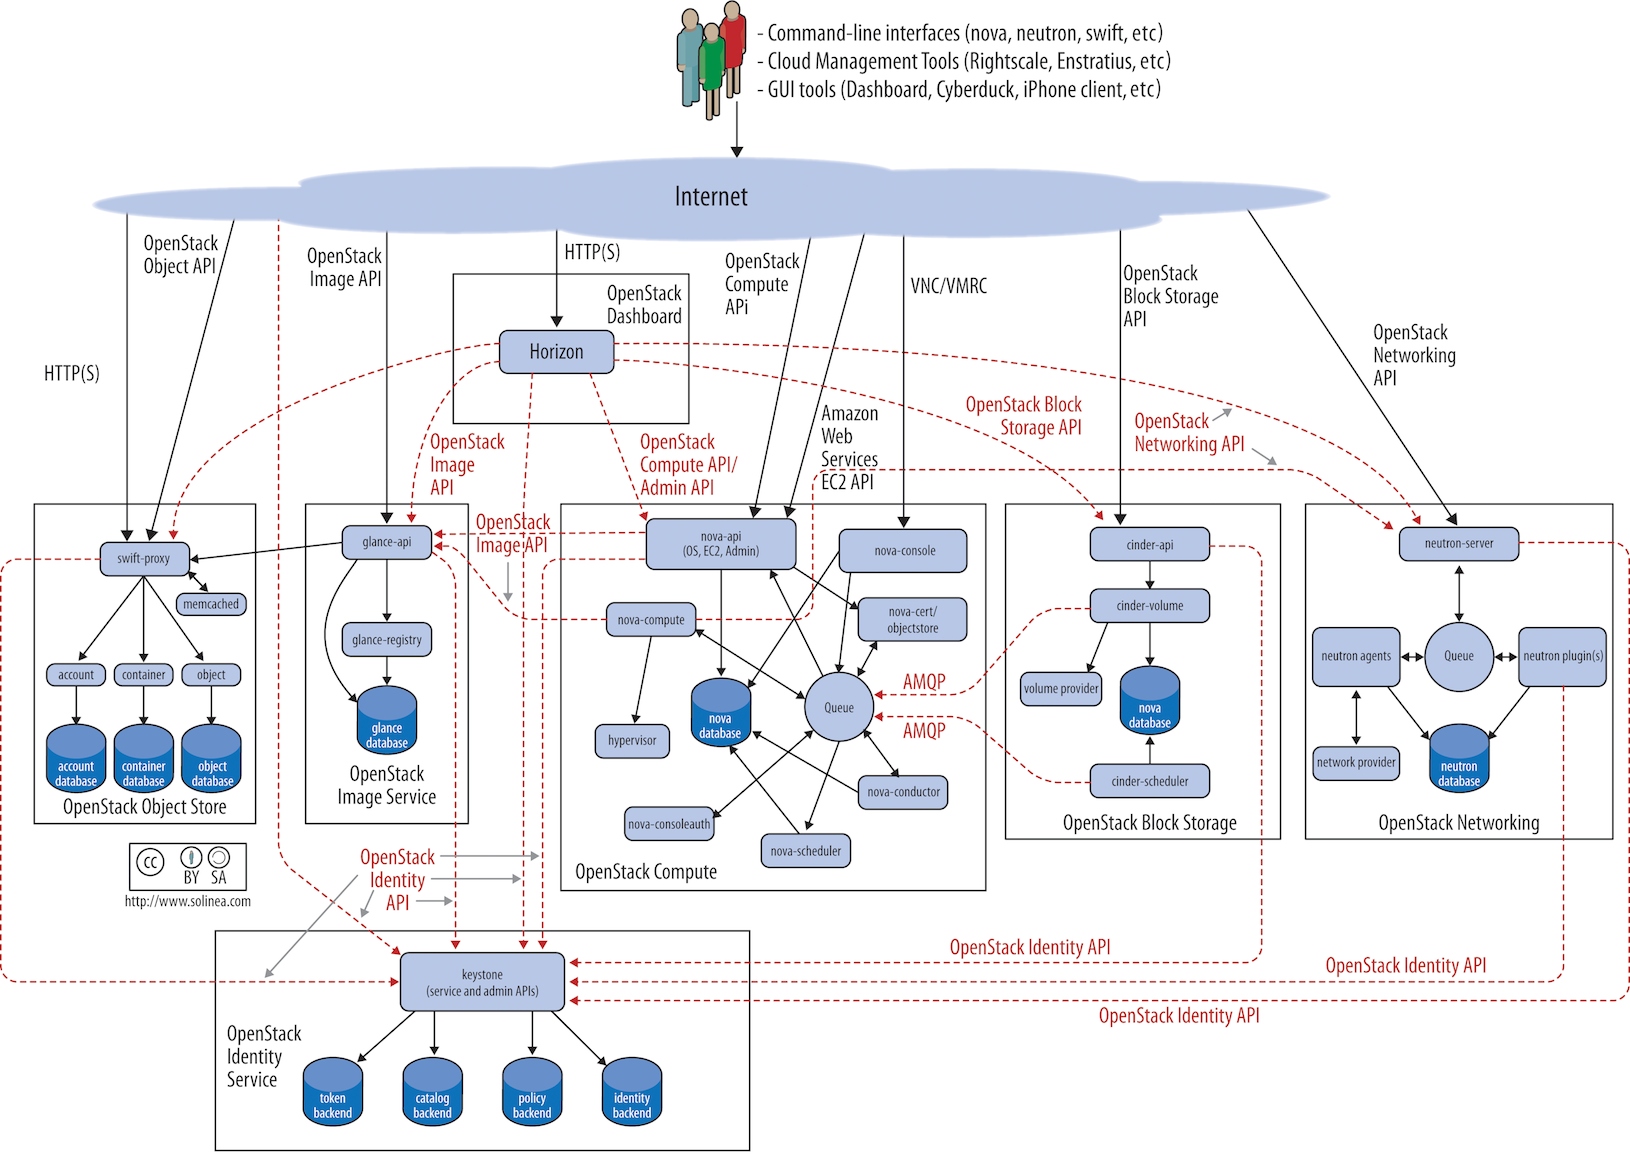
\includegraphics[width=0.9\textwidth]{openstack_logical}
